Cominciamo con lo sviluppare singolarmente ogni entità fondamentale in modo da approfondirne le caratteristiche principali. Quindi dalla visione generale entriamo nello specifico seguendo l'approccio misto precedentemente citato.\newline

\subsubsection{RICHIESTA SUL MEPA}
Il concetto di Richiesta sul MEPA raggruppa due entità, che sono il tipo di richiesta con cui la nostra azienda si interfaccia. In questo caso si parla di richieste di offerta sotto forma di Gara Pubblica oppure di Trattativa diretta.\newline In entrambi i casi abbiamo un numero univoco associato alla richiesta di offerta che la identifica, dobbiamo avere dei parametri fondamentali associati alla richiesta, che sono il limite di spesa specificato, il codice IPA e l'offerta proposta dalla nostra azienda a scopo statistico e le date di inizio e termine offerta.\newline
La richiesta sotto forma di gara pubblica avrà anche l'aggiudicatario della gara e la sua offerta, mentre la trattativa diretta dovrà definire se la trattativa è andata a buon fine attraverso l'attributo 'Stipulata'.\newline\newline
\noindent\makebox[\textwidth]{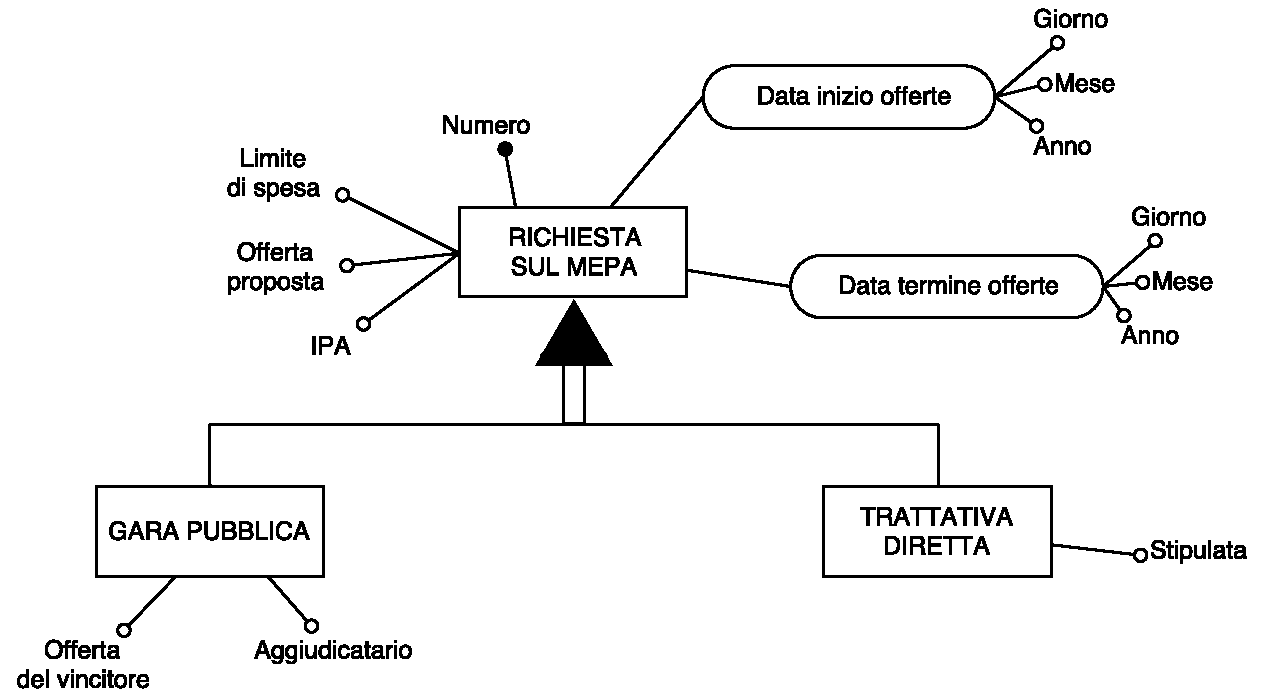
\includegraphics[width=0.9\linewidth]{./immagini/richiesta_sul_mepa.pdf}}

\subsubsection{PA O PERSONA O AZIENDA}
Questa entità raggruppa appunto le entità che hanno relazioni commerciali con la nostra azienda. Concettualmente c'è una doppia divisione, infatti l'entità fondamentale si divide in due entità quali il Fornitore e il Cliente. A sua volta l'entità cliente si divide in Pubblica Amministrazione, l'entità di maggior interesse, intorno alla quale si costruisce l'entità di Richiesta sul MEPA precedentemente descritta, e l'entità Privato, che è invece un cliente ordinario che può essere una persona o un'azienda.\newline
Tutte queste entità hanno bisogno di un codice identificativo, il codice PA nel caso delle pubbliche amministrazioni, il codice fiscale per le persone o la partita IVA per le aziende. In più viene tenuto in considerazione l'indirizzo pubblico PEC e la ragione sociale che contiene i dati dell'indirizzo (via, numero civico, città, CAP) e dati personali(nome, telefono, email).\newline
Vicino al fornitore è riportata l'entità dei costi di spedizone che non ha nulla a che fare con l'identità generale di pa, azienda o persona, ma è strettamente correlata al fornitore e va considerata, portando con se i dati riguardo il costo della spedizione, il peso e la somma delle misure massima e i tempi di consegna.
\newline\newline
\noindent\makebox[\textwidth]{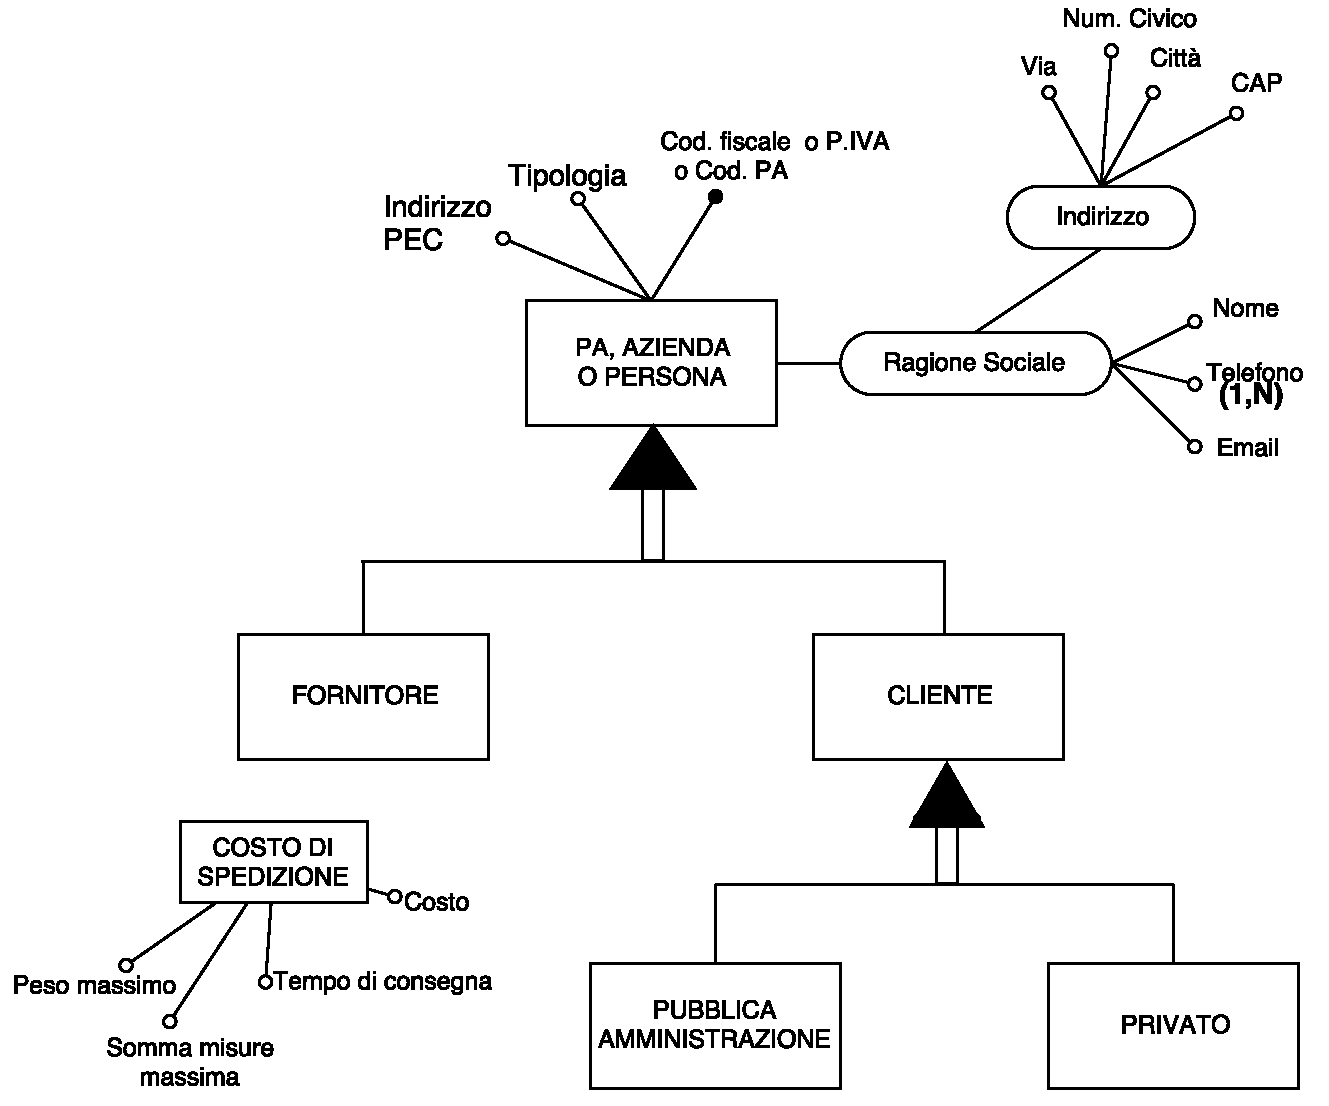
\includegraphics[width=0.7\linewidth]{./immagini/pa_persona_o_azienda.pdf}}

\subsubsection{PRODOTTO O SERVIZIO}
Questa identità raggruppa due identità molto diverse, il Prodotto e il Servizio, ed ha in comune soltanto il codice identificativo associato al prodotto o al servizio.\newline
Il prodotto è a sua volta un'entità che ne raggruppa molte altre, in particolare tutti i prodotti disponibili (Notebook, Memoria di Massa, RAM, Stampante, PC Desktop, Monitor, Cartuccia d'Inchiostro, Toner). Tutti questi prodotti devono avere indicati il produttore, il modello, le dimensioni e il peso, poi in base al prodotto in questione ognuno ha caratteristiche diverse rappresentate nei suoi attributi.\newline
D'altra parte il servizio è un entità singola particolare in quanto tra i suoi attributi ha il costo del servizio emesso e la tipologia, che descrive la prestazione effettuata. A tal proposito la descrizione del servizio deve essere standardizzata e necessita di particolare attenzione in quanto il servizio è solitamente descritto in maniera non univoca. \newline\newline
\noindent\makebox[\textwidth]{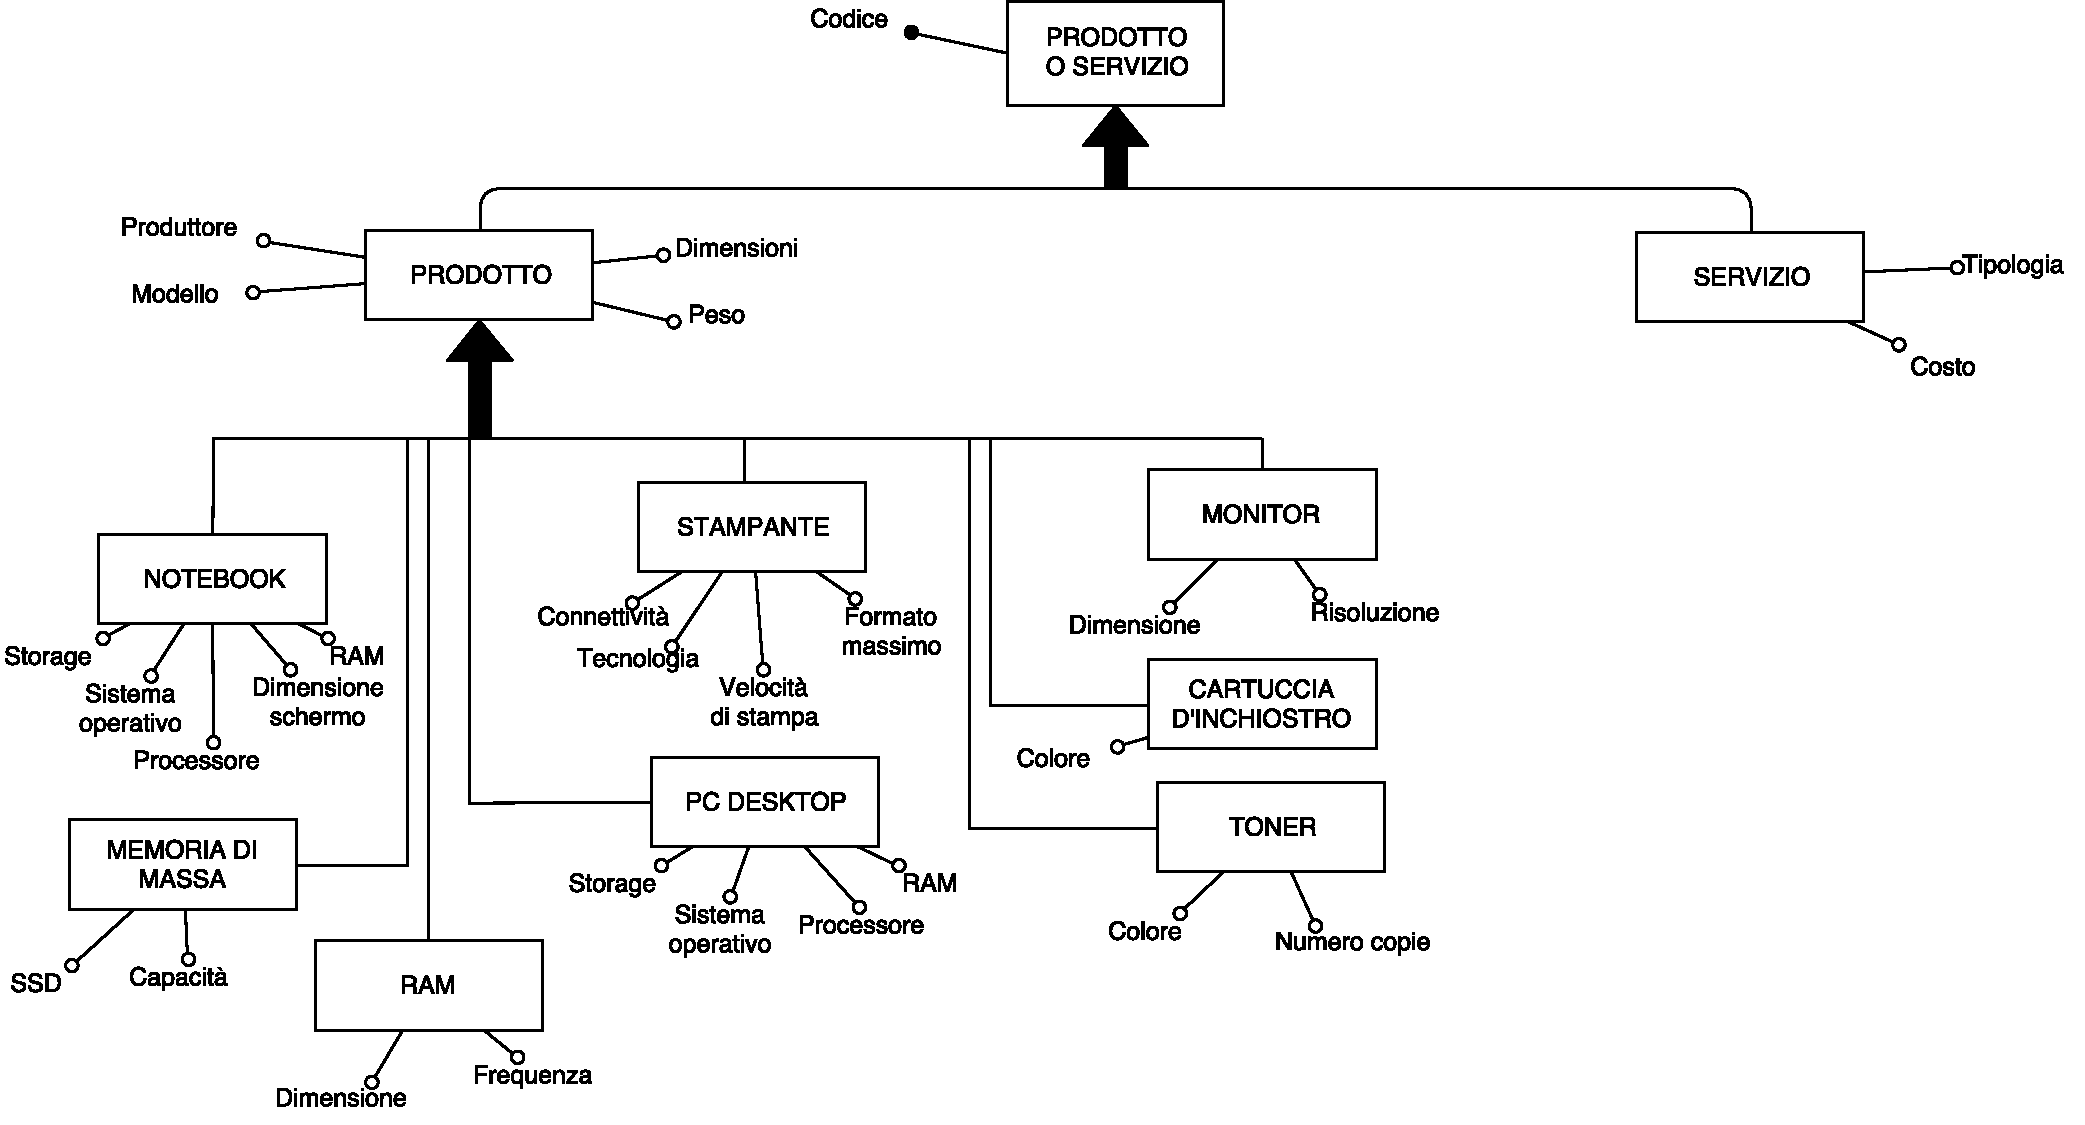
\includegraphics[width=0.9\linewidth]{./immagini/prodotto_servizio.pdf}}

\subsubsection{FATTURA}
L'entità della Fattura ha un ruolo centrale in quanto ad essa sono collegate tutte le operazioni effettuate dall'azienda, quindi acquisto dai fornitori oppure la vendita a privati o pubbliche amministrazioni.\newline
La fattura è identificata da un codice univoco, e le sue specifiche sono l'importo, l'emittente e il destinatario della fattura. In più sono riportate data di emissione, data di scadenza e data di pagamento.\newline
\noindent\makebox[\textwidth]{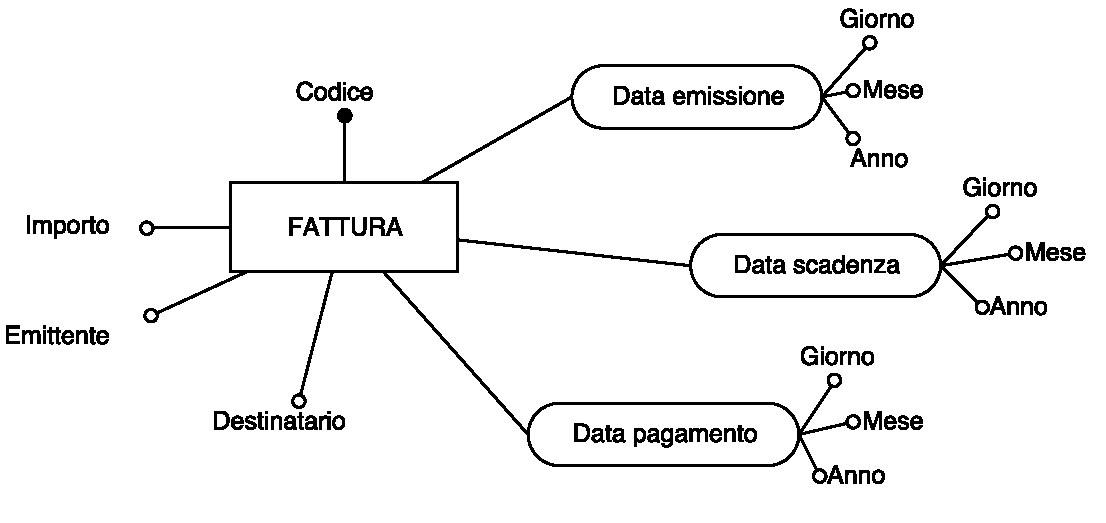
\includegraphics[width=0.7\linewidth]{./immagini/fattura.pdf}}
